% Options for packages loaded elsewhere
\PassOptionsToPackage{unicode}{hyperref}
\PassOptionsToPackage{hyphens}{url}
\documentclass[
]{ltjsarticle}
\usepackage{xcolor}
\usepackage[margin=20mm]{geometry}
\usepackage{amsmath,amssymb}
\setcounter{secnumdepth}{-\maxdimen} % remove section numbering
\usepackage{iftex}
\ifPDFTeX
  \usepackage[T1]{fontenc}
  \usepackage[utf8]{inputenc}
  \usepackage{textcomp} % provide euro and other symbols
\else % if luatex or xetex
  \usepackage{unicode-math} % this also loads fontspec
  \defaultfontfeatures{Scale=MatchLowercase}
  \defaultfontfeatures[\rmfamily]{Ligatures=TeX,Scale=1}
\fi
\usepackage{lmodern}
\ifPDFTeX\else
  % xetex/luatex font selection
\fi
% Use upquote if available, for straight quotes in verbatim environments
\IfFileExists{upquote.sty}{\usepackage{upquote}}{}
\IfFileExists{microtype.sty}{% use microtype if available
  \usepackage[]{microtype}
  \UseMicrotypeSet[protrusion]{basicmath} % disable protrusion for tt fonts
}{}
\makeatletter
\@ifundefined{KOMAClassName}{% if non-KOMA class
  \IfFileExists{parskip.sty}{%
    \usepackage{parskip}
  }{% else
    \setlength{\parindent}{0pt}
    \setlength{\parskip}{6pt plus 2pt minus 1pt}}
}{% if KOMA class
  \KOMAoptions{parskip=half}}
\makeatother
\usepackage{graphicx}
\makeatletter
\newsavebox\pandoc@box
\newcommand*\pandocbounded[1]{% scales image to fit in text height/width
  \sbox\pandoc@box{#1}%
  \Gscale@div\@tempa{\textheight}{\dimexpr\ht\pandoc@box+\dp\pandoc@box\relax}%
  \Gscale@div\@tempb{\linewidth}{\wd\pandoc@box}%
  \ifdim\@tempb\p@<\@tempa\p@\let\@tempa\@tempb\fi% select the smaller of both
  \ifdim\@tempa\p@<\p@\scalebox{\@tempa}{\usebox\pandoc@box}%
  \else\usebox{\pandoc@box}%
  \fi%
}
% Set default figure placement to htbp
\def\fps@figure{htbp}
\makeatother
\setlength{\emergencystretch}{3em} % prevent overfull lines
\providecommand{\tightlist}{%
  \setlength{\itemsep}{0pt}\setlength{\parskip}{0pt}}
\usepackage{bookmark}
\IfFileExists{xurl.sty}{\usepackage{xurl}}{} % add URL line breaks if available
\urlstyle{same}
\hypersetup{
  hidelinks,
  pdfcreator={LaTeX via pandoc}}

\author{}
\date{}

\begin{document}

\section{Paper 6: Conservation Laws, Records, and Time-like
Structure}\label{paper-6-conservation-laws-records-and-time-like-structure}

\subsection{\texorpdfstring{The \(\Sigma\lambda^2\) Non-conservation
Theorem, the Freezing Theorem, the \(B_4\) Gauge, the \(1{+}3\) Polar
Decomposition, the Record Theorem, and the Null
Structure}{The \textbackslash Sigma\textbackslash lambda\^{}2 Non-conservation Theorem, the Freezing Theorem, the B\_4 Gauge, the 1\{+\}3 Polar Decomposition, the Record Theorem, and the Null Structure}}\label{the-sigmalambda2-non-conservation-theorem-the-freezing-theorem-the-b_4-gauge-the-13-polar-decomposition-the-record-theorem-and-the-null-structure}

Author: Noriaki Kihara\\
Affiliation: WF System Co., Ltd.\\
ORCID: 0009-0004-6753-4020\\
Version: v0.3 (content and results unchanged from v0.2; nomenclature
unified to the displacement-record definition of Paper 0.5 ---
ledger/register sorted into displacement record / conserved quantity /
invariant / accounting. The λ side = displacement record, and the
direction (arrow of time) is attributed to the asymmetric one bit rather
than to monotonicity, consistent with Paper 0.5.)\\
Date: June 2026\\
DOI (this version): 10.5281/zenodo.20689914\\
Concept DOI: 10.5281/zenodo.20640456\\
License: CC BY 4.0

\begin{center}\rule{0.5\linewidth}{0.5pt}\end{center}

\subsection{Abstract}\label{abstract}

This paper establishes the kinematic core of the reciprocal dual model
(Papers 1--5). The assumptions are only three --- (1) the reciprocal
duality \(\nu\lambda=1\), (2) the zero point \(1/2\), and (3) one
asymmetric bit, namely that the additive conservation law rides on only
one of the two dual sides --- and this paper organizes, as theorems, how
much structure follows from this inventory.

First, the \textbf{freezing theorem}: under conservation of
\(\sum\nu^2\), every nontrivial split strictly increases
\(\sum\lambda^2\) (a one-line proof by Cauchy--Schwarz). As a corollary,
if both sums of squares were conserved simultaneously, no nontrivial
split would exist, and no cascade or time-like structure would arise.
\textbf{The existence of the asymmetric one bit is itself the existence
condition for time-like structure.}

Second, the \textbf{gauge structure}: the exact symmetry group of the
counting condition is the hyperoctahedral group \(B_4\) (order 384), and
within each energy shell the distribution over axes, the signs, and the
orientations are pure gauge. The additive conservation laws close the
accounting with just two entries, \(\sum\nu^2\) and the \(Z_2\) parity.
As a by-product, the fine structure of shells that are degenerate in
energy and split by shape (137 states at \(R=3\) \(\to\) 7
gauge-invariant classes) is laid bare.

Third, the \textbf{\(1{+}3\) polar decomposition}: it is not that one of
the four axes becomes time. In the polar decomposition
\(\mathbb{R}^4\cong\mathbb{R}_+\times S^3\) of the 4-dimensional
frequency space, the radial direction, on which the manifestation of the
asymmetric bit concentrates, appears as time-like, while the angular
directions untouched by the duality (the \(B_4\) gauge) appear as
space-like. The \(1{+}3\) role differentiation is obtained without
introducing the imaginary unit or the Minkowski negative sign. We also
show that there is no way to decide from the inside whether one is at
the apex of the hierarchy (hierarchy relativity).

Fourth, the \textbf{record theorem and the null structure}: measurement
is recording, and recording is accumulation. Since only a non-conserved
monotone quantity (the \(\lambda\) side) can accumulate, every
displacement record remains as a configuration on the \(\lambda\) side,
and \(\nu\) can never be a direct read-out target. The integer lattice
is reinterpreted not as an assumption but as the \textbf{resolution
structure of unit records} (a downgrade in the assumption inventory).
Furthermore, in the log-conjugate plane \((q,p)=(\log\lambda,\log\nu)\)
the constraint \(\nu\lambda=1\) is a \textbf{null line}, the freedom of
distributing the conjugate widths is the \(SO(1,1)\) boost (squeeze),
and uncertainty is built in as the boost-invariant minimal area. The
negative sign is not an axiom but a hyperbola --- though the aggregation
of the four pairs of \((1,1)\) structures into a single \((1,3)\)
signature remains as an explicit construction task.

This paper does not claim to have derived physical time, space, or
measurement. What it does claim is that, from the inventory of three
assumptions, the role differentiation into time-like, space-like,
record, uncertainty, and null structure follows as theorems.

\begin{center}\rule{0.5\linewidth}{0.5pt}\end{center}

\subsection{Keywords}\label{keywords}

conservation laws, arrow of time, records, relational time,
hyperoctahedral group, gauge redundancy, polar decomposition, null
structure, squeezing, uncertainty, hierarchy relativity

\begin{center}\rule{0.5\linewidth}{0.5pt}\end{center}

\subsection{1. Introduction}\label{introduction}

Through Paper 5 {[}3{]}, the mathematical foundation of the reciprocal
dual model (Paper 1 {[}1{]}, Paper 4 {[}2{]}) --- the dictionary, the
coherence conditions, and the classification of \(R^2\) --- was
established. The question of this paper is the following.

\begin{quote}
In this model, from which assumptions, and to what extent, does the
structure in which ``time appears to flow, space appears to extend, and
records appear to remain'' follow as theorems?
\end{quote}

The standpoint that does not regard time as a fundamental quantity but
constructs it from relations or records has a long lineage: the ``frozen
formalism'' in the canonical formulation of quantum gravity (DeWitt
{[}5{]}), time as conditional probability (Page \& Wootters {[}6{]}),
relational quantum mechanics (Rovelli {[}7{]}), the elimination of time
from dynamics (Barbour {[}8{]}), and quantum theory on a deterministic
substrate ('t Hooft {[}9{]}). This paper does not extend these theories;
its distinctive feature is that it implements the problem awareness that
``time is not fundamental'' as a family of theorems \textbf{exhaustively
verifiable within a finite lattice model}.

Organization of this paper: §3 treats the freezing theorem, §4 the
\(B_4\) gauge and the fine structure, §5 the \(1{+}3\) polar
decomposition and hierarchy relativity, §6 the record theorem, and §7
the null structure and uncertainty.

\begin{center}\rule{0.5\linewidth}{0.5pt}\end{center}

\subsection{2. Inventory of Assumptions}\label{inventory-of-assumptions}

The assumptions used in this paper are the following three (with
configuration reading and the record principle used jointly as operating
principles).

\begin{enumerate}
\def\labelenumi{\arabic{enumi}.}
\tightlist
\item
  \textbf{Reciprocal duality} \(\nu_n\lambda_n=1\).
\item
  \textbf{Zero point} \(1/2\) (structurally identified as the zero-point
  quantum in Paper 5).
\item
  \textbf{Asymmetric one bit}: the additive conservation law
  \(\sum\nu^2=S\) rides on one side only (the \(\nu\) side).
\end{enumerate}

An important remark: the labels \(\nu/\lambda\) in Assumption 3 are not
proper names but \textbf{markers of roles}. The assumption reduces to
the naming convention that the observer calls the side that appears
conserved the ``frequency,'' and the only remaining physical content is
the single bit that ``one asymmetry exists.'' The mirror model (calling
\(\sum\lambda^2\) the conserved quantity) is merely a relabeling of the
same structure.

\begin{center}\rule{0.5\linewidth}{0.5pt}\end{center}

\subsection{3. The Freezing Theorem: Asymmetry Is the Existence
Condition for Time-like
Structure}\label{the-freezing-theorem-asymmetry-is-the-existence-condition-for-time-like-structure}

\subsubsection{\texorpdfstring{3.1 The \(\Sigma\lambda^2\)
non-conservation
theorem}{3.1 The \textbackslash Sigma\textbackslash lambda\^{}2 non-conservation theorem}}\label{the-sigmalambda2-non-conservation-theorem}

\begin{quote}
\textbf{Theorem}: Under conservation of \(\sum\nu^2\) (\(s=\sum_a s_a\),
\(s_a\ge1\)), every nontrivial split (into \(n\ge2\) parts) strictly
increases \(\sum\lambda^2=\sum 1/s_a\).
\end{quote}

\textbf{Proof}: By Cauchy--Schwarz, \((\sum s_a)(\sum 1/s_a)\ge n^2\),
that is, \(\sum 1/s_a\ge n^2/s>1/s\) (for \(n\ge2\)). \(\blacksquare\)

Numerical confirmation over all 68 coherent partitions of odd \(s\le15\)
likewise shows no exception.

\begin{figure}
\centering
\pandocbounded{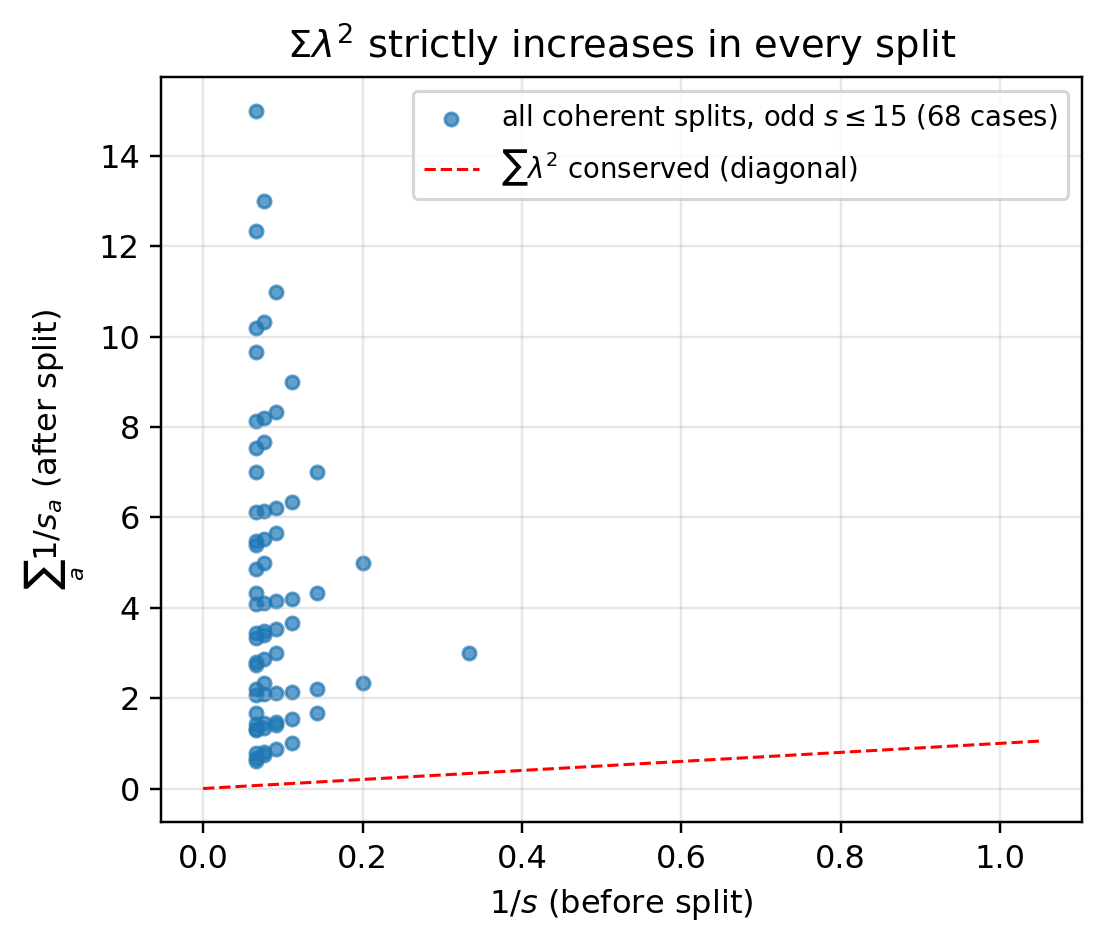
\includegraphics[keepaspectratio,alt={Figure 1. Strict monotonicity of the lambda side (displacement record) under every coherent split}]{figure_paper6_1_lambda_monotonicity.png}}
\caption{Figure 1. Strict monotonicity of the lambda side (displacement
record) under every coherent split}
\end{figure}

\textbf{Figure 1. The \(\Sigma\lambda^2\) monotone increase theorem: all
68 coherent partitions of odd \(s\le15\) lie above the diagonal (exact
computation).}

\subsubsection{3.2 The freezing theorem}\label{the-freezing-theorem}

\begin{quote}
\textbf{Corollary (freezing theorem)}: If both \(\sum\nu^2\) and
\(\sum\lambda^2\) were conservation laws, no nontrivial split would
exist at all, and no cascade, time-like structure, or expansion-like
structure would arise (the system freezes).
\end{quote}

That is, the fact that \(\sum\lambda^2\) is \textbf{not} conserved ---
the existence of the asymmetric one bit --- is itself the condition
under which time-like structure can exist. The \(\lambda\) side (the
displacement record) is the only monotone quantity in this model, and
its monotone increase provides time-like structure (the possibility
condition for ordering); the direction --- the ``arrow of time'' itself
--- does not follow from monotonicity alone but is attributed to the
asymmetric one bit of which dual side the conservation law rides on
(consistent with Paper 0.5). Note that whereas the classical
correspondence between symmetries and conservation laws (Noether
{[}4{]}) determines \emph{what} is conserved, the asymmetric one bit
here is an independent choice of \emph{which dual side the conservation
law rides on}.

\subsubsection{3.3 Invariance under dual
relabeling}\label{invariance-under-dual-relabeling}

In log space the duality is the point symmetry \(p=-q\), and the
kinematic content of the splitting cascade (ratios, exponents,
dimensionless quantities) is invariant under the relabeling
\(\nu\leftrightarrow\lambda\). The only element that does not disappear
under the relabeling is the single bit of ``which side is additive,''
and this is the precise content of Assumption 3 in §2.

\begin{center}\rule{0.5\linewidth}{0.5pt}\end{center}

\subsection{\texorpdfstring{4. The \(B_4\) Gauge Structure and the Fine
Structure of
Shells}{4. The B\_4 Gauge Structure and the Fine Structure of Shells}}\label{the-b_4-gauge-structure-and-the-fine-structure-of-shells}

\subsubsection{4.1 Symmetry group and orbit
decomposition}\label{symmetry-group-and-orbit-decomposition}

The exact symmetry group of the counting condition
\(\sum(|k_i|+\tfrac12)^2\le R^2\) is the hyperoctahedral group \(B_4\)
(signed permutations of the coordinates, of order \(2^4\cdot4!=384\);
for the general theory see Humphreys {[}10{]}). The \(B_4\) orbits of
shell \(m\) are labeled by the shape (the multiset of the \(|k_i|\)),
and the orbit size is given by

\[
|\mathcal{O}(\text{shape})|=\frac{4!}{\prod_v m_v!}\times 2^{\#\{i:|k_i|>0\}}
\]

(verified to agree with the shell counts for all shells with
\(m\le25\)).

\subsubsection{4.2 Gauge nature and closure of the
accounting}\label{gauge-nature-and-closure-of-the-accounting}

Within each orbit, \(B_4\) acts transitively. Therefore the distribution
over axes, the signs, and which axes are excited are \textbf{pure gauge}
--- they are carried into one another by lattice rotations --- and
require no fixing by conservation laws.

\begin{quote}
\textbf{Closure of the accounting}: The non-gauge content of a state
consists of the two items \((m,\text{shape})\). The additive
conservation laws are exactly two --- \(\sum\nu^2\) and the \(Z_2\)
parity (Paper 5) --- and the accounting of degrees of freedom closes.
\end{quote}

\subsubsection{4.3 Fine structure of
shells}\label{fine-structure-of-shells}

The structure of shells degenerate in energy (\(m\)) and split by shape
first appears at \(m=7\) (\(40=32+8\)). The number of states after gauge
reduction is 7 at \(R=3\) and 27 at \(R=5\), dramatically smaller than
the nominal capacities (137, 1545). These ``shape multiplets'' will play
the role of physical quantum numbers in subsequent papers.

\begin{figure}
\centering
\pandocbounded{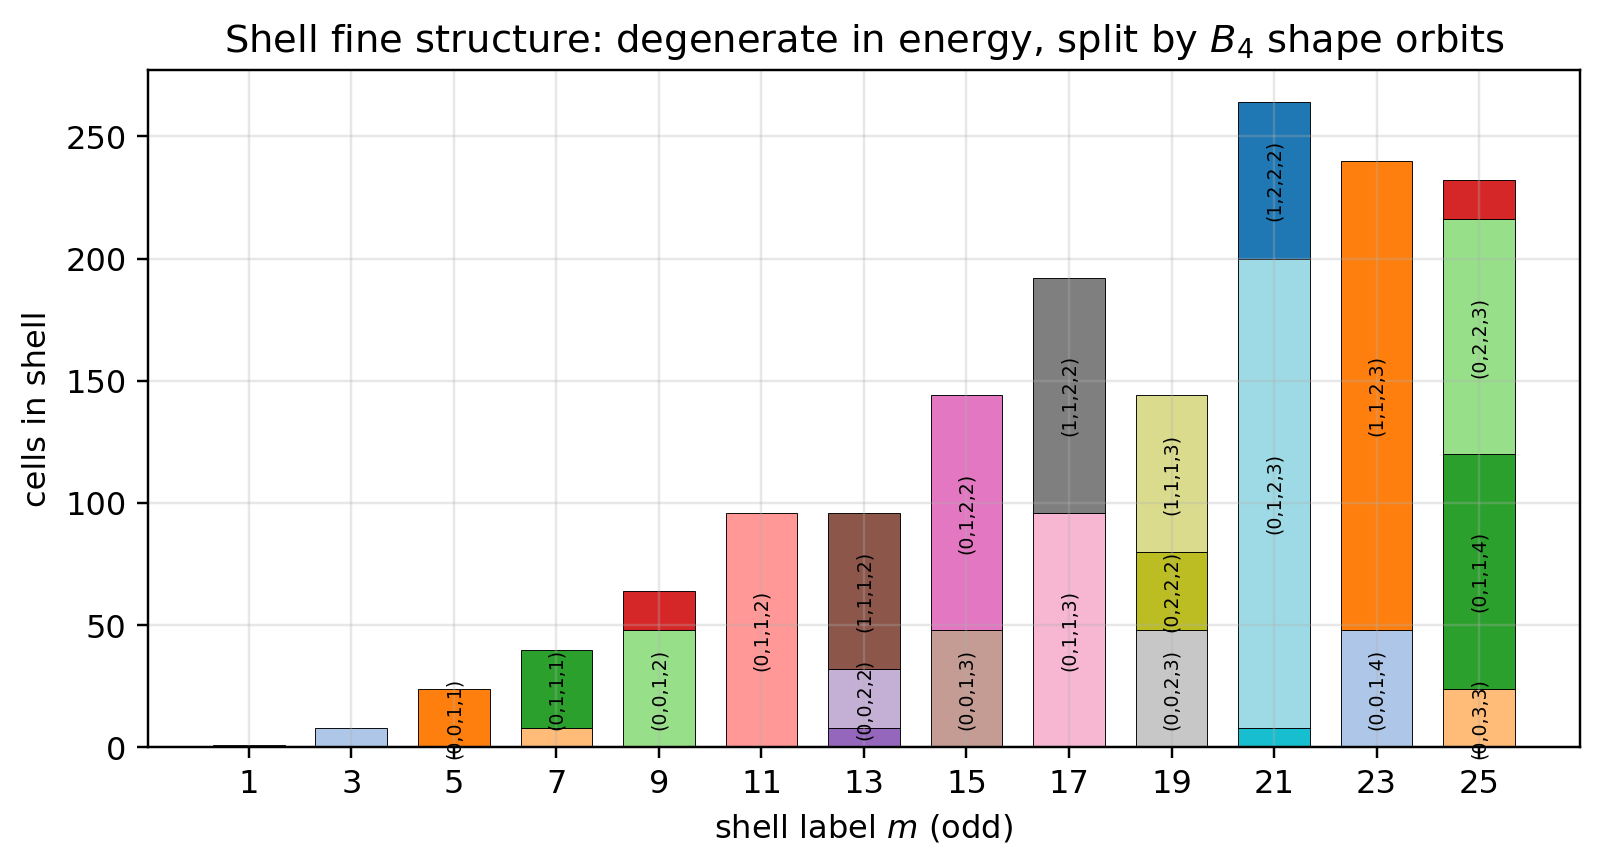
\includegraphics[keepaspectratio,alt={Figure 2. B4 shell fine structure}]{figure_paper6_2_B4_shell_structure.png}}
\caption{Figure 2. B4 shell fine structure}
\end{figure}

\textbf{Figure 2. \(B_4\) shell fine structure (exhaustive for
\(m\le25\)): shells degenerate in energy split into shape orbits (first
splitting at \(m=7\)).}

\begin{center}\rule{0.5\linewidth}{0.5pt}\end{center}

\subsection{\texorpdfstring{5. The \(1{+}3\) Polar Decomposition and
Hierarchy
Relativity}{5. The 1\{+\}3 Polar Decomposition and Hierarchy Relativity}}\label{the-13-polar-decomposition-and-hierarchy-relativity}

\subsubsection{5.1 Radial = time-like, angular =
space-like}\label{radial-time-like-angular-space-like}

In the polar decomposition
\(\mathbb{R}^4_\nu\cong\mathbb{R}_+\times S^3\) of the 4-dimensional
frequency space:

\begin{itemize}
\tightlist
\item
  \textbf{Radial direction}: the internal clock \(\tau=1/R'\) is a
  function of the radius alone, and the motion of the splitting cascade
  is purely radial. Within a hierarchy level, the manifestation of the
  asymmetric bit concentrates on the radial quantity \(R'\). Hence
  time-like.
\item
  \textbf{Angular directions}: the shell degeneracy is a discretized
  \(S^3\), and the angular degrees of freedom are the \(B_4\) gauge (§4)
  --- neither energy nor clock. The log-space duality \(p=-q\) preserves
  the structure of the radial lines and does not touch the angles. Hence
  space-like.
\end{itemize}

\begin{quote}
The \(B_4\) symmetry of the four axes is never broken. What is
``broken'' is not an axis but a different way of slicing: radial versus
angular. The role of the complex phase is taken over by the cos/sin
doubling of the real standing-wave dictionary, and the role of the
Minkowski negative sign by the null structure of §7 --- \textbf{neither
the imaginary unit nor the negative sign is introduced}.
\end{quote}

\subsubsection{5.2 Intrinsic distortion}\label{intrinsic-distortion}

The zero point \(1/2\) strictly breaks metric flatness: it produces an
effective boundary (the Weyl term, Paper 5 §4) on a torus that has no
boundary, and necessarily creates an unfilled layer around every state.
A perfectly flat state space is the zero-point-free limit, and no state
can exist there. \textbf{To exist and to be distorted are the same
condition.}

\subsubsection{5.3 Hierarchy relativity}\label{hierarchy-relativity}

Viewed from one hierarchy level above, the whole system is
indistinguishable from an ordinary cell with the same spectrum (odd
numbers, Paper 5), the same zero point, and a single representative
label. Therefore:

\begin{quote}
There is no way to determine from the inside that one is at the apex of
the hierarchy. The distinction between ``whole'' and ``part'' is a
hierarchy-indexical term, not a structural attribute.
\end{quote}

The only absolute scale is the zero point \(1/2\), the minimal cell, and
this closes self-referentially in the form that the lowest level of the
hierarchy defines the unit. All observables of an internal observer are
ratios, and the structure is completely relational.

\begin{center}\rule{0.5\linewidth}{0.5pt}\end{center}

\subsection{6. The Record Theorem}\label{the-record-theorem}

\subsubsection{6.1 Theorem}\label{theorem}

Measurement is recording, and recording is accumulation. Only a
non-conserved, monotone quantity (the displacement record) can
accumulate. By the theorem of §3:

\begin{itemize}
\tightlist
\item
  \(\sum\nu^2\): invariant under all splits (exchange only is possible;
  accumulation is impossible).
\item
  \(\sum\lambda^2\): the only monotone quantity (the displacement
  record), strictly increasing under all splits.
\end{itemize}

\begin{quote}
\textbf{Corollary (record theorem)}: Every measurement record can only
remain as a configuration on the \(\lambda\) side. \(\nu\) can be
estimated only via exchange and counting, and can never be a direct
read-out target.
\end{quote}

The reason for the von Neumann-type observation {[}11{]} that every
actual measurement terminates in a position reading (the location of a
pointer, a photographic plate, a detector) appears in this model as a
theorem.

\subsubsection{6.2 Integer lattice = resolution structure (downgrading
an
assumption)}\label{integer-lattice-resolution-structure-downgrading-an-assumption}

The overlap for discriminating a frequency difference \(\Delta\nu\)
within an observation window \(T\) is
\(|\mathrm{sinc}(\pi\Delta\nu T)|\), and the resolution is
\(\delta\nu=1/T\). \(\nu\) cannot be read in a snapshot; the price is
duration. Since, with the unit record window \(T=1\), discrimination
becomes exact precisely for \textbf{integer differences}:

\begin{quote}
The integer \(\nu\) lattice is reinterpreted not as an assumption about
\(\nu\), but as \textbf{the structure of what a unit record can
resolve}.
\end{quote}

\begin{center}\rule{0.5\linewidth}{0.5pt}\end{center}

\subsection{\texorpdfstring{7. The Null Structure: \(\nu\lambda=1\) Is
the Light Cone of the Log-Conjugate
Plane}{7. The Null Structure: \textbackslash nu\textbackslash lambda=1 Is the Light Cone of the Log-Conjugate Plane}}\label{the-null-structure-nulambda1-is-the-light-cone-of-the-log-conjugate-plane}

\subsubsection{7.1 Null line and boosts}\label{null-line-and-boosts}

Taking \((q,p)=(\log\lambda,\log\nu)\) for each conjugate pair,
\(\nu\lambda=1\iff u\equiv q+p=0\). \textbf{The constraint is a null
line.} The cascade --- the time-like motion --- is translation along
this null line (the \(v=q-p\) direction), while the direction off the
cone (\(u\)) is frozen at the zero point and is paid only as
uncertainty.

The freedom of distributing the conjugate widths,
\(S_\eta:(\delta_\nu,\delta_\lambda)\to(e^{-\eta}\delta_\nu,e^{\eta}\delta_\lambda)\),
strictly preserves the area \(\delta_\nu\delta_\lambda\), and this is
precisely the \(SO(1,1)\) hyperbolic rotation --- the \textbf{boost} ---
of the \((u,v)\) plane.

\subsubsection{7.2 Uncertainty = boost-invariant minimal
area}\label{uncertainty-boost-invariant-minimal-area}

The boost invariant is the area, and its minimal value is the zero point
\(1/2\).

\begin{quote}
The structure corresponding to the uncertainty principle is built in as
the \textbf{boost-invariant minimal cell} of the \((1,1)\) geometry. The
negative sign is not an axiom but a hyperbola.
\end{quote}

\begin{figure}
\centering
\pandocbounded{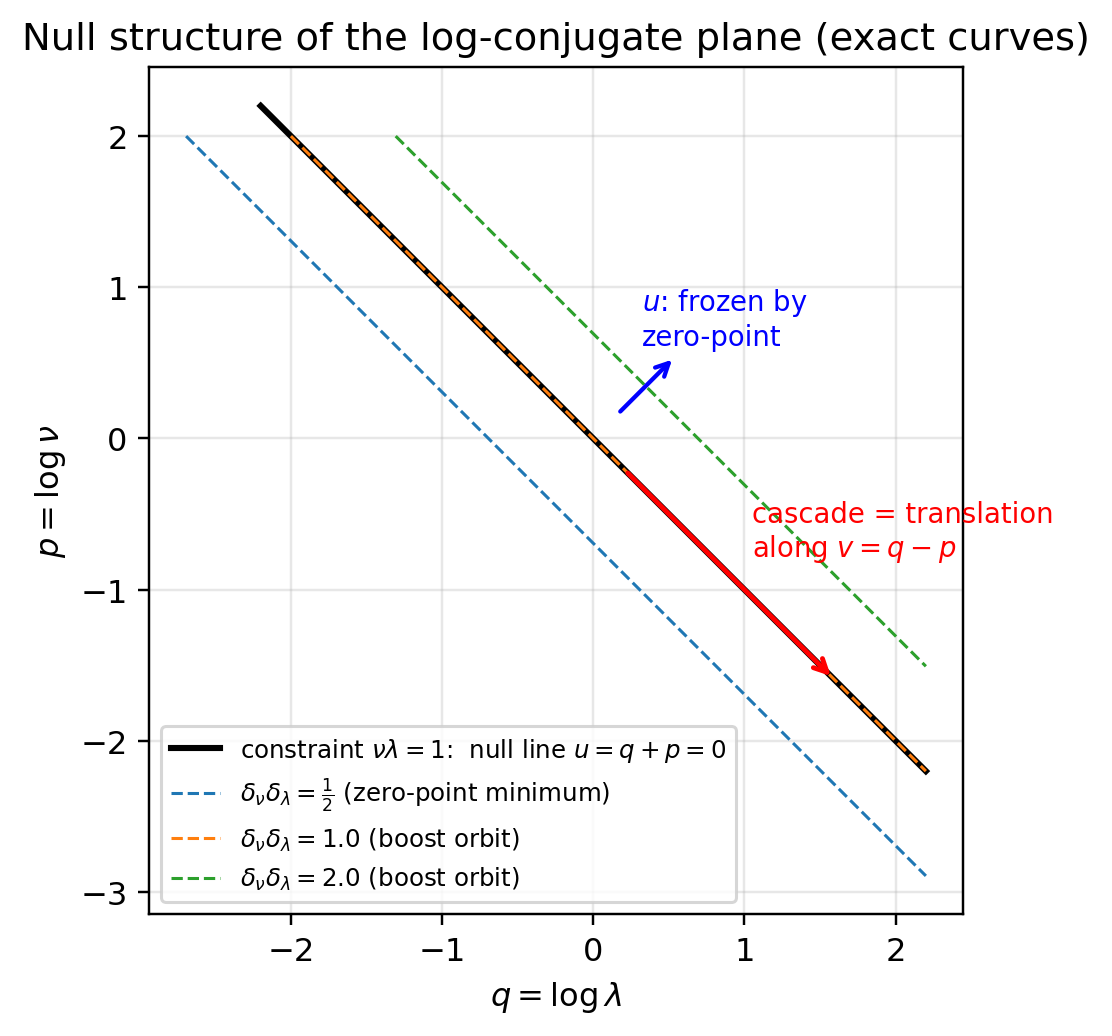
\includegraphics[keepaspectratio,alt={Figure 3. Null structure of the log-conjugate plane (exact curves)}]{figure_paper6_3_null_structure.png}}
\caption{Figure 3. Null structure of the log-conjugate plane (exact
curves)}
\end{figure}

\textbf{Figure 3. Null structure of the log-conjugate plane (exact
curves): the constraint \(\nu\lambda=1\) is a null line, the
distribution freedom consists of boost orbits (hyperbolas), and the
minimal area is the zero point \(1/2\).}

\subsubsection{7.3 What remains explicitly
unconstructed}\label{what-remains-explicitly-unconstructed}

The \((1,1)\) null/boost structure derived in §7 exists \textbf{per
conjugate pair} (\((1,1)^{\times4}\)). Assembling it into a single
\((1,3)\) Minkowski signature requires a specification that aggregates a
single time direction out of the four pairs; the natural candidate is
the radial direction (§5), but the explicit construction of the
aggregation map is outside the scope of this paper. We note in passing
that, even in special relativity, the \((1,3)\) signature and the
dimensionality themselves are empirical inputs, not derived results.

\begin{center}\rule{0.5\linewidth}{0.5pt}\end{center}

\subsection{8. Scope of Claims of This
Paper}\label{scope-of-claims-of-this-paper}

What this paper claims: (1) the \(\Sigma\lambda^2\) non-conservation
theorem and the freezing theorem (with proof); (2) the asymmetric one
bit = the existence condition for time-like structure; (3) the \(B_4\)
gauge nature, the closure of the accounting, and the fine structure of
shells (exhaustively verified); (4) the \(1{+}3\) polar decomposition
(radial = time-like, angular = space-like) and hierarchy relativity; (5)
the record theorem and the reinterpretation of the integer lattice as a
resolution structure; (6) the null structure, boosts, and the invariant
area (per pair).

What this paper does not claim: (1) the derivation of physical time,
space, or measurement; (2) the construction of the \((1,3)\) Minkowski
metric; (3) a continuous action of the Lorentz group; (4) any extension
or modification of the theories of relational time {[}5--9{]}. The terms
``time-like'' and ``space-like'' are restricted to describing the role
differentiation within the model.

\begin{center}\rule{0.5\linewidth}{0.5pt}\end{center}

\subsection{9. Conclusion}\label{conclusion}

From the three assumptions (\(\nu\lambda=1\), the zero point \(1/2\),
and the asymmetric one bit), the following follow as theorems with no
additional assumptions: (i) the existence condition for time-like
structure (the freezing theorem); (ii) the gauge nature of the
space-like degrees of freedom (\(B_4\)); (iii) the \(1{+}3\) role
differentiation (the polar decomposition); (iv) the asymmetry of records
(the record theorem); and (v) the geometry of uncertainty (the null
structure and the invariant area). The direction of time, the
accumulation of records, and the asymmetry of metrizability are all
different faces of one and the same single bit.

With the integer lattice downgraded from an assumption to a resolution
structure, the assumption inventory of the model has become lighter
still. The subsequent papers build, on top of this kinematic core, the
configuration statistics (Paper 7), the two accountings (Paper 8), and
the stability of composites (Paper 9).

\begin{center}\rule{0.5\linewidth}{0.5pt}\end{center}

\subsection{Appendix: Essentials of the Reproduction
Procedure}\label{appendix-essentials-of-the-reproduction-procedure}

The numerical confirmation of \(\Sigma\lambda^2\) non-conservation
covers all 68 coherent partitions of odd \(s\le15\); the \(B_4\) orbit
decomposition is checked by classifying all cells with \(|k_i|\le6\) and
comparing against the orbit-size formula (\(m\le25\)); the sinc
discrimination table is evaluated on the grid
\(\Delta\nu, T\in\{0.25,\ldots,4\}\); squeeze invariance is confirmed to
machine precision for 5 random pairs. Scripts and research notes are
provided in the public repository
(https://github.com/WurabeSeiji/ai-chat-logs-open).

\begin{center}\rule{0.5\linewidth}{0.5pt}\end{center}

\subsection{References}\label{references}

{[}1{]} Noriaki Kihara, Paper 1, v0.3, 2026. Concept DOI:
10.5281/zenodo.20588036.

{[}2{]} Noriaki Kihara, Paper 4, v1.0, 2026. Concept DOI:
10.5281/zenodo.20638962.

{[}3{]} Noriaki Kihara, ``Paper 5: The Cell--Standing-Wave Dictionary
and the Quantization of the Radius,'' v0.2, 2026. Concept DOI:
10.5281/zenodo.20640454.

{[}4{]} E. Noether, ``Invariante Variationsprobleme,'' Nachr. Königl.
Ges. Wiss. Göttingen (1918), 235--257.

{[}5{]} B. S. DeWitt, ``Quantum theory of gravity. I. The canonical
theory,'' Physical Review 160 (1967), 1113--1148.

{[}6{]} D. N. Page and W. K. Wootters, ``Evolution without evolution:
Dynamics described by stationary observables,'' Physical Review D 27
(1983), 2885--2892.

{[}7{]} C. Rovelli, ``Relational quantum mechanics,'' International
Journal of Theoretical Physics 35 (1996), 1637--1678.

{[}8{]} J. Barbour, \emph{The End of Time}, Oxford University Press,
1999.

{[}9{]} G. 't Hooft, \emph{The Cellular Automaton Interpretation of
Quantum Mechanics}, Springer, 2016.

{[}10{]} J. E. Humphreys, \emph{Reflection Groups and Coxeter Groups},
Cambridge University Press, 1990.

{[}11{]} J. von Neumann, \emph{Mathematische Grundlagen der
Quantenmechanik}, Springer, 1932.

\begin{center}\rule{0.5\linewidth}{0.5pt}\end{center}

\subsection{License}\label{license}

This paper is published under CC BY 4.0.\\
Reuse, adaptation, translation, and citation are permitted, provided
that the author name, version, publication date, and source are clearly
indicated.

\end{document}
